\documentclass[11pt,twocolumn]{article}
%\documentclass{article}

\usepackage{appendix}
\usepackage{graphicx}
\usepackage{hyperref}

\def\thetitle{Human Computer Interaction 2011/2012 \\ Coursework 2}
\def\theauthor{Stephen McGruer (s0840449) and Wenqi Yao(s0838969)}

% TITLE PAGE
\title{\thetitle}
\author{\theauthor}
\date{\today}

\begin{document}

\maketitle
\thispagestyle{empty}

\section{Introduction}

In this paper, we evaluate the application \emph{Tag App} by comparing it against Nielsen's usability heuristics, as well as conducting cooperative and natural user testing. These results are combined with our previous evaluation of the MIT \emph{LabelMe} interface to identify key strengths, weaknesses, and improvements for our own application \emph{Image Labeller}.

\section{Initial Evaluation}

We first applied Nielsen's usability heuristics\cite{nielsen1994} to determine \emph{Tag App}'s strong and weak areas, and to identify problems that users would likely come up against.

\subsection{Key Strengths}

One strength that we found was the visibility of changes in the system status - five of the seven buttons gave clear visual feedback. The application also avoided using overly technical language, and supported recognition-based over recall-based interaction (avoiding hidden options or menus.) A help file was made available, with concrete steps for users to follow. Finally, it had a
clean and minimalistic design with no unnecessary options, although the chosen colour scheme (orange and yellow) might not be appealing to all users. 

\subsection{Key Limitations}

\indent \indent Placement of and feedback from buttons was not ideal. In particular, clicking the `Save' button disabled it without confirmation of the change in system status (e.g. an `image saved' pop-up). The `Open' and 'Save' buttons, which affect the entire image, were mixed with buttons such as `New', which only affects a single label. This is illustrated in {\bf Figure 1}. Additionally, the `Help' button, which plays a key role in user guidance, was not in an eye-catching position.

\begin{figure}[h!]
\centering
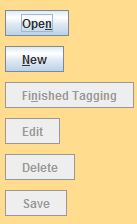
\includegraphics[scale=0.8]{buttonpanel.png}
\caption{Button panel, showcasing inconsistent grouping. `Help' is not on the button panel.}
\end{figure}

There was also a lack of consistency and accuracy in the use of language. Labels were referred to at different points as `objects' and `labels', while the act of adding a label was referred to as `adding an object', `creating a label', and `tagging an object'. The `Edit' button's actual function was to rename the selected label.

There was poor support for user control. Keyboard shortcuts or application preferences could not be set, even though letters in some names were underlined corresponding to the general standards for shortcuts (e.g. `Ope\underline{n}'). The shortcut \emph{Alt-N} opened the Help file, but this was never documented, suggesting that it was unintentional.

Finally, the application was inflexible towards many possible changes in users' decisions. Global undo/redo functionality was not available. Also, there was no option to cancel label creation after providing a name, so the only way to stop creating a label was to finish it. Right clicking while drawing a label would undo the last point; however, this functionality was not intuitive. 

\subsection{Bugs Found}

\begin{itemize}
\item \emph{Clicking the `Delete' button while multiple labels were selected} would only delete one label. The `Delete' and `Edit' buttons would be left disabled, so other labels could not be deleted or renamed.
\item \emph{Clicking the `Home' button in the `Open Image' dialogue} would disable the `up' arrow, leaving the dialogue stuck in the `home' folder.
\end{itemize}

\section{User Evaluation}

\subsection{Methodology}

We used two types of evaluation methods to test the software; Cooperative Evaluation and Natural Evaluation. 

\emph{ Selecting Subjects.} Nielsen and Landauer suggest that using three to five subjects yields the maximum benefit to cost ratio\cite{nielsen1993}. However, Nielsen also argues that when novices evaluate an application, around 14 subjects are needed to identify 75\% of problems \cite{nielsen19932}. As \emph{Tag App} has limited functionality, we decided that a smaller number of subjects would not affect results greatly, and it was more important to maximise our cost-benefit. Hence, we used five subjects for cooperative evaluation, and four for natural evaluation. We selected a mix of male and female users from a variety of backgrounds to represent the intended user base. A short description of each user can be found in {\bf Appendix A: User Descriptions}.

\emph{Procedure.} Before testing the software, users were briefed on the aims of our project, as well as the rationale behind creating applications for labelling images. The `Thinking-Aloud' technique was explained in order to facilitate dialogue between the user and experimenter, and to disambiguate users’ actions. Users were also told about the experiment procedure, and informed that they might withdraw their participation at any time. After the evaluation, users were asked for feedback on aspects of the program that confused them, and for suggestions on improving the interface.

\emph{Recording Results.} Subjects' actions and comments were noted by hand. As stated in our previous report, differences in subjects' reading speed and memory of the tasks given would affect the time taken for them to accomplish each task. These timings were therefore not recorded. Quantitative data was instead taken from subjects' rating of the application, as well as the number of subjects who performed each action.

\subsubsection{Cooperative Evaluation}

Testing was carried out in small rooms in Appleton Tower on the University DICE machines. Users were given a list of six tasks to complete in order: 

\begin{enumerate}
\item Labelling one object in a scene
\item Opening an image from a different folder
\item Labelling multiple objects in a scene
\item Deleting objects
\item Editing the area of a label
\item Closing the program
\end{enumerate}
 
These six tasks covered all functionality in the program, except (1) undoing a point while creating a label, and (2) renaming a label. After each user completed Task 3, they were prompted by the experimenter to rename labels, through the use of simple scenarios (e.g. "What if a machine doesn't know that `Hut 1' and `Hut 2' are both the same kind of object?"). Not explicitly asking the users to carry out these tasks is in line with Molich's \cite{molich} testing guidelines, which states that users should be given goals, rather than steps or descriptions. The task sheet given to users can be found in {\bf Appendix B: User Tasks}.

After completing the tasks, users were given a short survey about their experience completing each task. The questions from this survey can be found in {\bf Appendix C: User Survey}.

\subsubsection{Natural Evaluation}

To make the evaluation setting resemble environments that a user would normally be in, the program was run on a Windows environment (rather than Linux) on laptops, in a range of different locations. Each user was provided with a sample image to label, but given free rein to import any images from other folders, as well as create any labels that they wanted to.  

\subsection{Results}

\subsubsection{Cooperative Evaluation}

Subjects found it difficult to accomplish the given tasks, with one user describing the program as `very demanding on users'. The subjects scored each task out of 5, with 1 being the lowest and 5 being the highest. They found it easiest to select (4.6pts) and delete (4.4pts) labels; while opening an image (2.6pts) was deemed the hardest task, followed by label editing (3.0pts) and then creating a label (3.2pts).

While all subjects were able to save and close the image, they ran into a multitude of other problems:
 
\textbf{Unintuitive Interface.} None of the subjects managed to create a label on their first try, or load an image without assistance. To create a label they attempted a variety of methods including clicking directly on the image (four subjects) and clicking the `Open' button (two subjects). To load an image, every subject tried to click the location bar to change the directory, and three subjects tried to click the `File Type' field. Additionally, one subject tried to click the `Home' button when opening a new image, locking the loading dialog in a state where buttons no longer worked. Finally, when creating more labels in Task 3, two subjects replicated mistakes that they had made earlier. 

\textbf{Poor Documentation.} All subjects were prompted to check the help file when stuck, but this was not always useful. After reading the documentation, one subject tried to right-click to undo points, but was confused by the colours of the lines changing arbitrarily. Another subject did not understand the instruction `add vertices to the image panel', as she did not know what the
image panel was. Subjects also did not always use the same language as the help documentation - for example, one subject searched the section titled `Delete Label' instead of looking for `undo' as they wanted to `delete the last line [they] drew'.

\textbf{Bugs \& Inflexibility.} One subject made a spelling error in naming a label. Since they could not cancel or rename the label within the label creation state, they decided to `make it and then delete it later'. Also, all of the subjects created multiple labels with the same name. Since all of these labels were highlighted when any were selected, two users accidentally deleted the wrong label.

\subsubsection{Natural Evaluation}

A 10 minute time frame was suggested for subjects to explore \emph{Tag App}. On average, subjects spent 13 minutes and 20 seconds using the application, though this was skewed by an enthusiastic subject who used it for 20 minutes and 3 seconds.

The table below shows each feature that we identified in the program, and the number of subjects who successfully used it.

\begin{table}[h!]
\centering
\begin{tabular}{|l|c|}
\hline
{\bf Feature } & {\bf \# } \\ 
\hline
Opening a new image & 3 \\
Creating a new label & 4 \\
Undoing points during label creation & 0 \\
Renaming a label & 2 \\
Deleting a label & 1 \\
Saving an image & 4 \\
Using the help file & 2 \\
\hline
\end{tabular}
\caption{\# of subjects who used each feature.}
\label{features}
\end{table}
 
Subjects also made several errors, mostly due to misconceptions about the program. These are detailed in the next table:

\begin{table}[h!]
\centering
\begin{tabular}{|l|c|}
\hline
{\bf Error/Misconception} & {\bf \#} \\
\hline
{\bf Changing folder to open image} - & \\
\emph{Location/File Type} bars clicked & 4 \\
\emph{`Home'} icon clicked & 2 \\
\hline
{\bf Creating a new label} - & \\
\emph{`Open'} clicked to start new label & 2 \\
\emph{Cursor dragged} instead of clicked & \\
to create points & 1 \\
\hline
{\bf Edit label points:} `Edit' clicked & 2 \\
\hline
{\bf Accidents:} Clicked `Delete' for `Edit' & 1 \\
\hline
\end{tabular}
\caption{\# of subjects who made each error.}
\label{errors}
\end{table}

Furthermore, subjects did not always understand the program output, as shown below.

\begin{table}[h!]
\centering
\begin{tabular}{|l|c|}
\hline
{\bf Aspect causing confusion} & {\bf \#} \\
\hline
Changing of label colours & 2 \\
Highlighting of selected labels & 2 \\
Vocabulary: `vertices' for points & 2 \\
Multiple labels with the same name & 2 \\
\hline
\end{tabular}
\caption{\# of subjects confused by each aspect.}
\label{confusion}
\end{table}

{\bf Gaps in Analysis}. Even though we utilised the `Thinking-Aloud' method, it was not always possible to identify subjects’ intents. One subject commented `I want to draw a box around the lamp', and promptly clicked the `Open' button. It was unclear if two
of the subjects meant to create a new label when they clicked `New', as they were clicking the buttons systematically from top to bottom.

We were unable to test the usefulness of the help documentation during natural evaluation. Two subjects did not click the `Help' button, attributing this to `never us[ing] the help file' when working with other programs. One subject only noticed it halfway during the evaluation, and the final subject did not find extra functionality from reading it.

\subsubsection{Bugs}

Two subjects found new bugs in the application. 
\begin{itemize}
\item \emph{Clicking the 'X' button on the `Save Image?' dialog} acts as if you clicked `No' rather than `Cancel', so any subsequent dialogs (such as the Open Image dialog) appear
anyway, without feedback about the state. 
\item \emph{ Opening a non-image file} crashes the application.
\end{itemize}

\noindent Full results can be found in \textbf{Appendix D: Full User Evaluation Results}

\section{Discussion of Results}

We found that our hypotheses (based on Nielsen's heuristics) were generally
mirrored by the actions and thoughts of the subjects involved in our two
evaluations. However, there were some cases where feedback did not match our
predictions. In this section we discuss these discrepancies between theory and
practice, and suggest corresponding improvements.

As expected, subjects seemed to seek out and respond to changes in the system
state. They saw and interacted with pop-up dialogues displayed after they
clicked a button, and were confused by the lack of feedback from the `Save'
functionality, especially during the transition between the `Do you want to
save?' and `Open Image' dialogues. 

However, at least four subjects did not make the link between a label being
highlighted and it being selected. This might be due to the change in various
visual cues when a label is selected: the arbitrary changes in the colours of
non-selected labels could detract from the thick, bright red line of a selected
label. This problem could be reduced by tying each label to a particular
colour, or colouring each label by its current state (e.g. Selected).

Lack of consistency did cause confusion around the act of `labelling/tagging'
and the button functionality. However, we failed to recognise several words
that were used that might not be suitable for users. For example, a user was
confused by a reference to the `Image Panel' in the help documentation, as the
meaning of this phrase was never defined. Ways to mitigate this include
renaming the buttons (e.g. changing `New' to `New Label', `Finished Tagging' to
`Finished Labelling') as well as including a help graphic which points out the
names and locations of different panels.

Subjects had trouble repeating previous tasks that they had performed, showing
that they had to recall action sequences rather than immediately recognise
what to do next. One noted that this behaviour was due to the ambiguously named
buttons. The renaming of buttons as suggested above would help to alleviate
this problem. 
 
Contrary to our expectations, subjects struggled to use the help documentation.
Problems included finding the section in the help file that was appropriate to
their problem, and the general wording of the documentation. While three
subjects used the help documentation to learn about the undo functionality, two
others mentioned wanting to undo points, but did not find the corresponding
section in the documentation. The documentation might benefit from an FAQ list,
as there were many common questions such as `How do I make a line?'

Subjects replicated many of the bugs that we found. One wanted to cancel the
label that he had just started creating, but was unable to do so. This problem
would be easily eliminated with the addition of a `Cancel' button. Four
subjects locked the `Open Image' dialogue in a state where only the current
folder could be accessed, since they could not understand many buttons and
fields in the dialogue. No subjects triggered the multiple-label-delete
error, possibly due to the limited time spent and labels made.

\subsection{User Suggestions}

Subjects in both evaluations made several suggestions, all of which could be
valuable additions to the application. However, due to development costs and
characteristics of the intended user base, we found some improvements to be
more critical than others.

\subsubsection{Functional Aspects}

One user thought that having the cursor hover over a label on the image should
cause the name of the label to appear. This would increase the users mental
link between a label and its name, making it easier to select a label from the
list. Two users thought it would be useful to draw curves - we previously
thought of this while developing our own application, but found it too
difficult to implement. Two subjects opened images that were not ideally sized,
prompting them to suggest zoom or resizing functionality. This would be a good
addition to the program if unusually sized images were expected, although the
high cost of implementing a zoom functionality means that we would suggest
resizing images instead.

\subsubsection{Linguistic aspects}

One user mentioned that the button names were ambiguous, as `New' could mean
either `New Label' or `New Image', and suggested that we make them more
specific. Additionally, two users were confused by the use of both `labels' and
`tagging' in the application. As we have mentioned above, we think reducing the
ambiguity in \emph{Tag App} is very important, and as such would consider this a
necessary change for the application. Another user was confused by the use of
the word `vertices' in the context of what she considered `putting dots'
(before she created enough to see a line). As only one user had problems with
this use of language, we consider that `vertices' is not too technical a word,
and we would continue to use it.

\section{Comparative Evaluation}

To identify key improvements for our application \emph{Image Labeller}, we compared it against both our new \emph{Tag App} discoveries and a previous analytical evaluation of MIT’s \emph{LabelMe}\footnote{See our previous
report}.\\

\noindent \emph{Image Labeller} was inferior to other the applications in three main areas:

\textbf{Recognition-based Interfaces.} In \emph{Tag App} and \emph{LabelMe}, all available actions are contained on the screen (with the exception of \emph{Tag App}’s `Undo'). While the main actions within \emph{Image Labeller} are always visible,
others are hidden in the menu-bar and the user must remember which menu they are in. 

\textbf{Visual Links and Indicators.} When a label is selected, \emph{Tag App}
highlights it with a thick red line and \emph{LabelMe} shades the area contained by
its edges. While \emph{Image Labeller} does change the colour of the selected label,
this is not as clear as the other two applications. When creating a label, a
useful function in \emph{LabelMe} is the large marker indicating the first point
added. Neither \emph{Tag App} nor \emph{Image Labeller} offer such a feature.

\textbf{Use of Technical Language.} Most instructions in \emph{Tag App} and
\emph{LabelMe} use simple, non-technical language. However, the concept of
`Collections' in \emph{Image Labeller} may be considered too abstract for the novice
user. \\

\noindent Some problems in \emph{Tag App} and \emph{LabelMe} revealed similar issues
in \emph{Image Labeller}:

\textbf{Poor Help Documentation.} Both \emph{Tag App} and \emph{Image Labeller} have
help functions that are often overlooked. \emph{LabelMe} uses its help documentation
as a landing page, at the expense of making the actual application hard to
find. 

\textbf{Ambiguous Buttons.} All three applications suffer from some
ambiguity in their button names; \emph{Tag App} for almost all buttons, \emph{LabelMe} in the
`Erase' button, and \emph{Image Labeller} in its icon-based buttons. \\

\noindent Other problems in \emph{Tag App} and \emph{LabelMe} highlighted positive aspects of
\emph{Image Labeller}:

\textbf{Display of Available Actions.} In \emph{Tag App}, one can click the
`Delete' button when more than one label is selected, even though only one
label will be deleted. The labels that remain cannot be selected for deletion.
\emph{LabelMe} allows the user to click the `Erase' button even when nothing can be
erased. On the other hand, actions that might lead to the user being trapped in
a particular state have been disabled in \emph{Image Labeller}. \\

Based on our comparison, we came up with five changes we would make to Image
Labeller:

\textbf{Implementation of an Icon-Bar.} Icon-based shortcuts for actions such as `Save' would promote recognition-based interaction.

 \textbf{Shading of Selected Label Area.} Increased visibility of selected labels would strengthen users' mental link between label names and corresponding areas.

\textbf{Enlarged First Points in Label Creation.} The lack of this feature did not hinder subjects during iterative development tests. However, the increased clarity from a larger first point would be well worth the small cost of implementation.

\textbf{Addition of a Tutorial.} As suggested by one of the subjects from our natural evaluation, users could be familiarised with the application with a tutorial that appeared on their first visit.

\textbf{Reducing Button Ambiguity.} Studies have shown that \emph{user-preferred} names overlap by only 15-35\% \cite{furnas1987}. However, to maximise the clarity of our button names and icons, we would like to run a study to find the best \emph{user-understood} names and pictures, even if these would not be the first-choice names for most users.  

\section{Conclusion}

Nielsen's usability heuristics were effective in helping us identify many of \emph{Tag App}'s limitations, as shown by the strong correlation between the aspects we highlighted and the issues faced by real users during testing. However, results from user evaluation were crucial in aiding our understanding of the extent of each problem. With this deeper knowledge of the impact of strengths and limitations in \emph{Tag App} on real users, it was possible to identify a set of improvements in \emph{Image Labeller} that would optimise user benefit while minimising the extra cost of development.

\begin{thebibliography}{9}

\bibitem{nielsen1994}
  Nielsen, J.,
  \emph{Enhancing the explanatory power of usability heuristics}.
  Proceedings of the ACM CHI'94 Conference,
  1994

\bibitem{nielsen1993}
  Nielsen, J., and Landauer, T.K.,
  \emph{A mathematical model of the finding of usability problems}.
  Proceedings of ACM INTERCHI'93 Conference, pp. 206-213,
  1993

\bibitem{nielsen19932}
  Nielsen, J.,
  \emph{Usability Engineering}.
  Academic Press, pp. 156,
  1993

\bibitem{molich}
  Molich, R.,
 \emph{230 Tips and Tricks for a Better Usability Test}.
  Nielsen Norman Group,
  2001

\bibitem{furnas1987}
 Furnas, G. W., Landauer, T. K., Gomez, L. M., Dumais, S. T.,
 \emph{The Vocabulary Problem in Human-System Communication}. 
  Communications of the ACM, 30 (11), 964-971.,
  1987

\end{thebibliography}

\onecolumn

\appendix
\appendixpage

\section{User Descriptions}

\subsection{Cooperative Evaluation}

\begin{itemize}
\item User 1 is a 22 year old female and a 4th year Biology graduate.
\item User 2 is a 20 year old female and a 2nd year undergraduate Law student. 
\item User 3 is an 18 year old female and a 1st year undergraduate Politics with Geography student. 
\item User 4 is a 22 year old male and a postgraduate Linguistics student. 
\item User 5 is a 22 year old female working in biomedical research. 
\end{itemize}

\subsection{Natural Evaluation}

\begin{itemize}
\item User A is a 22 year old male and a 3rd year undergraduate Pharmacology student. Testing was carried out at a desk in a bedroom.
\item User B is a 21 year old female and a 4th year undergraduate History student. Testing was carried at a sofa in an open area of Appleton Tower.
\item User C is a 21 year old female and a 4th year undergraduate Spanish and English Literature student. Testing was carried out at a desk in room 5.07 of Appleton Tower.
\item User D is a 22 year old male and a Biology graduate working in a watch store. Testing was carried out at a desk in his home. 
\end{itemize}

\newpage
\section{User Tasks}
\underline{\bf User Evaluation} \newline

\noindent In this evaluation, you will be testing some software for labelling images (i.e. for indicating what region of an image contains what objects). You will be asked to label a few images, and afterwards will be asked a few general questions about your opinion on the software. \newline 

\noindent {\bf Task \#1}

You should see a picture of a Hut. 
\begin{itemize}
\item Please label the hut ``Hut".
\item Save the image.
\end{itemize}

\noindent {\bf Task \#2} 
\indent \indent \indent \indent \indent \indent  \indent \indent \indent  \indent \indent \indent \indent \indent \indent 
\indent  \indent \indent \indent \indent  \indent \indent \indent 
\emph{I’m a nut, that’s not a real hut!}

You are currently in the folder {\bf /HCI/Eval/images}.
\begin{itemize}
\item Please open the image ``huts.jpg" from the folder {\bf /HCI/Images}.
\end{itemize}

\noindent {\bf Task \#3}
\indent \indent \indent \indent \indent \indent 
\indent  \indent \indent \indent \indent  \indent \indent \indent  \emph{A machine will need some luck to find these hut[s]...}
\begin{itemize}
\item Please label every hut in the image you have just loaded.
\end{itemize}

\noindent {\bf Task \#4} \indent \indent \indent \indent \indent \indent  \indent \indent \indent  \indent \indent \indent \indent
\indent \indent \indent \indent \indent \indent \emph{One hut (or more) won’t make your cut.}
\begin{itemize}
\item Please delete the 2 huts you dislike the most.
\end{itemize}

\noindent {\bf Task \#5} \indent \indent
\indent \indent \indent \indent \indent \indent  \indent \indent \indent  \indent \indent \indent \indent \indent \indent 
\indent  \indent \indent \indent \indent  \indent \indent \indent  \emph{Did we forget a little jut?}
\begin{itemize}
\item Please reload the first image, ``hut.jpg" from the folder {\bf /HCI/Eval/images}.
\item Ensure that your label covers the signboard outside the store.
\end{itemize}

\noindent {\bf Task \#6}
\begin{itemize}
\item Please close the program.
\end{itemize}

\newpage
\section{User Survey}

This survey was given as an online form. Users were asked to rate each aspect of the program on a scale of 1 to 5, where 5 was the best score (e.g. task was easiest to accomplish). 

\subsection{Survey Questions}

\begin{enumerate}
\item How easy was it to OPEN an image? 
\item How easy was it to CREATE a label?
\item How easy was it to SELECT a label?
\item How easy was it to EDIT a label? 
\item How easy was it to DELETE a label?
\item How AESTHETICALLY PLEASING was the software?
\end{enumerate}

\subsection{Online Survey}

The online survey can be found on:\\ \url{http://docs.google.com/spreadsheet/viewform?hl=en_US&formkey=dG1PSWZQX1M0ZkFrNVJ4WXhHcm5CTEE6MQ#gid=0}

\newpage
\section{Full User Evaluation Results}

This appendix contains the full results from each of our user evaluations.

\subsection{Cooperative Evaluation}

\textbf{User A}
\begin{itemize}
\item Task \#1: Labelling the Hut
\begin{itemize}
\item Was not sure where or how to start labelling.
\item Tried to click on the image (without clicking `New').
\item Tried to click on `Open'.
\item Prompted to use the help documentation. 
\item Clicked `New'.
\item Didn't know what to do then - rechecked help without prompting.
\item Managed to label the hut. Tried to finish by clicking on starting point.
\item Saved without trouble.. 
\end{itemize}
\item Task \#2: Opening a Picture
\begin{itemize}
\item Clicked `Open' immediately. 
\item Did not know how to get to the correct folder. 
\item Prompted to use the up arrow, and eventually found image without further help. 
\end{itemize}
\item Task \#3: Labelling Many Huts
\begin{itemize}
\item Tried to label multiple huts at once.
\item Did not use `undo' to correc the mistake; deleted and re-did instead.
\end{itemize}
\item Task \#4: Deleting Huts
\begin{itemize}
\item No issues.
\end{itemize}
\item Task \#5: Editing the Area of a Label
\begin{itemize}
\item Asked if she had to select the label, delete it, and draw a new one.
\item Researcher confirmed that this was true.
\item No other issues.
\end{itemize}
\item Task \#6: Closing the Program
\begin{itemize}
\item Found the close option in the top-left menu without trouble.
\item Asked researcher whether this was the right option.
\end{itemize}
\item Extra Comments
\begin{itemize}
\item Thought that the name of a label should appear if she moused over it.
\end{itemize}
\end{itemize}

\textbf{User B}
\begin{itemize}
\item Task \#1: Labelling the Hut
\begin{itemize}
\item Did not know how to label the hut.
\item Tried to click in labels box.
\item Tried to click on `Open'.
\item Prompted to use the help documentation. 
\item Clicked `New'.
\item Immediately clicked `Finished Tagging'.
\item When this didn't work, opened the help documentation again.
\item Confused by the mention of an `image panel'.
\item Tried to move frame to look for the image panel.
\item Clicked randomly on the image, causing points to appear.
\item Tried to drag the points around.
\item `I don't get this.'
\end{itemize}
\item Task \#2: Opening a Picture
\begin{itemize}
\item Clicked `Open' immediately. 
\item Did not realise folder had to be changed, did not know what to do.
\item Opened help documentation again, did not find answer.
\item Researcher helped user find the correct folder.
\end{itemize}
\item Task \#3: Labelling Many Huts
\begin{itemize}
\item Tried to drag points as before.
\item Checked the help documentation again.
\item Randomly clicked points, attempting to draw a large box around the general area of the hut.
\item Checked the help documentation, realised there was an `undo' feature.
\item Undid most of her random points, and managed to draw around each hut.
\item Renamed the huts quickly without trouble.
\end{itemize}
\item Task \#4: Deleting Huts
\begin{itemize}
\item Tried clicking on the labels on the image to select them.
\item No other issues.
\end{itemize}
\item Task \#5: Editing the Area of a Label
\begin{itemize}
\item Tried to select a label and right click to `undo' points.
\item Tried clicking `Edit'.
\item Realised she had to delete and make a new label.
\end{itemize}
\item Task \#6: Closing the Program
\begin{itemize}
\item Unsure about where to click; guessed correctly and confirmed with researcher.
\end{itemize}
\item Extra Comments
\begin{itemize}
\item Wanted to click and drag a box around an object.
\item Didn't know what she was saving when she clicked `Save'.
\item Noted help documentation is not consistent: `label' versus `tagging'.
\end{itemize}
\end{itemize}

\textbf{User C}
\begin{itemize}
\item Task \#1: Labelling the Hut
\begin{itemize}
\item Tried to click on the image, noted that nothing happened.
\item Discovered the `New' button.
\item No other issues.
\end{itemize}
\item Task \#2: Opening a Picture
\begin{itemize}
\item Clicked `Open' immediately. 
\item Did not know how to change the folder.
\item Researcher helped user find the correct folder.
\end{itemize}
\item Task \#3: Labelling Many Huts
\begin{itemize}
\item Wanted to `undo' while labelling, but termed it `delete [my] last line'.
\item Searched help documentation for `delete` and didn't find the `undo' functionality.
\item Finished label, deleted it, and redrew it instead.
\item No other issues.
\end{itemize}
\item Task \#4: Deleting Huts
\begin{itemize}
\item Did not know which hut was selected, as all were named the same.
\item Guessed at the hut they wanted, got it wrong.
\end{itemize}
\item Task \#5: Editing the Area of a Label
\begin{itemize}
\item Clicked `Open' to re-open the first image.
\item The `Do you want to save?' dialog appeared.
\item Did not understand what it was about; clicked the close button.
\item (Due to a bug) the `Open' dialog appeared anyway, with no feedback.
\item User commented: `I don't know what I just did'.
\item Once the correct image was opened, tried to edit points by clicking on existing label and then on image.
\item When nothing happened, deleted old label and drew a new one instead.
\end{itemize}
\item Task \#6: Closing the Program
\begin{itemize}
\item No issues.
\end{itemize}
\item Extra Comments
\begin{itemize}
\item Expected that clicking on the starting point of a label would finish the creation.
\item Found navigating between folders `impossible'.
\item Found that editing was `impossible'.
\end{itemize}
\end{itemize}

\textbf{User D}
\begin{itemize}
\item Task \#1: Labelling the Hut
\begin{itemize}
\item Tried to click straight on the image to add points.
\item Tried to click the label box to add points.
\item Tried to click `Open' to add points.
\item Then tried `New'.
\item Asked `Can I undo?' - researcher prompted user to check help documentation.
\item Found the feature in the help documentation.
\item Right clicked a few times while adding points, but was confused by the lines changing colour.
\end{itemize}
\item Task \#2: Opening a Picture
\begin{itemize}
\item Clicked `Open' immediately.
\item Did not know how to change directory.
\item Activated the `Home' bug, and so was instructed by the researcher how to proceed.
\end{itemize}
\item Task \#3: Labelling Many Huts
\begin{itemize}
\item Tried to click `Open' to add new points/
\item Moused over `New' and waited for the tooltip.
\item No other issues.
\end{itemize}
\item Task \#4: Deleting Huts
\begin{itemize}
\item Did not seem to notice that labels were highlighted when their names were clicked.
\item Deleted huts just by referring to the labels box.
\end{itemize}
\item Task \#5: Editing the Area of a Label
\begin{itemize}
\item Closed the program instead of opening the other image.
\item Did not know whether to click `Edit' or to click `New'.
\item Tried to click `Edit' and move points.
\item No other issues.
\end{itemize}
\item Task \#6: Closing the Program
\begin{itemize}
\item No issues.
\end{itemize}
\item Extra Comments
\begin{itemize}
\item Found the application `very demanding on users'.
\end{itemize}
\end{itemize}

\textbf{User E}
\begin{itemize}
\item Task \#1: Labelling the Hut
\begin{itemize}
\item Tried to click on the image to add points, multiple times.
\item Tried to click the label box to add points.
\item Tried to click on the disabled buttons.
\item Tried to drag on the image to draw a line.
\item Found the help documentation and read the whole document.
\item No other issues.
\end{itemize}
\item Task \#2: Opening a Picture
\begin{itemize}
\item Did not know how to change directory.
\item Found correct folder with help of researcher.
\end{itemize}
\item Task \#3: Labelling Many Huts
\begin{itemize}
\item Named a label incorrectly, and couldnt find a way to change the name while editing.
\item Finished the label, deleted it, and recreated it instead.
\item No other issues.
\end{itemize}
\item Task \#4: Deleting Huts
\begin{itemize}
\item Tried to click on the image to select labels.
\item Deleted the wrong huts due to the labels having the same name.
\end{itemize}
\item Task \#5: Editing the Area of a Label
\begin{itemize}
\item Tried to click the `Edit' button.
\item Tried to drag points.
\item Tried to click the `Edit' button and then drag points.
\item Checked the help documentation.
\item Tried to right click to undo points.
\item No other issues.
\end{itemize}
\item Task \#6: Closing the Program
\begin{itemize}
\item No issues.
\end{itemize}
\item Extra Comments
\begin{itemize}
\item Thought that `New' was an ambiguous name.
\end{itemize}
\end{itemize}

\subsection{Natural Evaluation}

\textbf{User A}
\begin{itemize}
\item Clicked `Open' to add points initially.
\item Clicked `New', then didn't know how to proceed.
\item Tried clicking `Edit' and `Finished Tagging'.
\item Read the error dialogue from `Finished Tagging', realised how to add points.
\item Tried to change the colour of a label using the `Edit' button.
\item Noted: `All I can do is change the name'.
\item Tried to open a new image. Struggled to change folder, but eventually worked it out.
\item Selected a label and noticed that it highlighted in red.
\item After about 6 minutes, noted `I can't find anymore functions'.
\item Tried to edit a label by clicking `New'.
\item Tried to use one name for multiple labels: `How do I make them together?'
\item Tried to change point location while creating a label.
\item Interview Comments
\begin{itemize}
\item Suggested that it should be possible to undo points, undo objects, and add curved lines.
\item Found the button text ambiguous.
\item Wanted zoom functionality.
\item Didn't think to use the help file, as `I never use help'.
\end{itemize}
\end{itemize}

\textbf{User B}
\begin{itemize}
\item Immediately started with `Open', and opened the same image that they already had open.
\item Next tried `New'.
\item Clicked on the centre of the object they wanted to label, and was surprised to see a point appear.
\item Tried to click `Finished Tagging'.
\item Read the `not enough vertices' error and realised how to add labels.
\item Tagged the objects correctly, except for the first point (did not undo it.)
\item Tried to finish tagging by clicking on the start point.
\item Hit `Open' to open another image, and the save prompt appeared.
\item Mistook the Open Image dialogue for a Save Dialogue. 
\item Noticed `Help' button, and noted that they had not noticed it before due to its location.
\item After 7 minutes, user was `bored' with the task.
\item Tried to open another image, and activated the home button bug.
\item Gave up as they couldn't now open another image.
\item Finished after 9 minutes as user was bored.
\item Interview Comments
\begin{itemize}
\item Wanted a tutorial, as they didn't know where to start.
\end{itemize}
\end{itemize}

\textbf{User C}
\begin{itemize}
\item Clicked `New', but was unsure how to use it.
\item Tried dragging (`I can't draw it', `This is ridiculous').
\item Clicked, and a point appeared.
\item Continued to click, alternating left and right (causing points to appear and be undone.)
\item Eventually realised she did not need to right click, and finished a label.
\item Was surprised when clicking on label names caused all labels to change colour.
\item Tried to `create a new image' but instead renamed her car label.
\item Struggled to open a new image.
\item Noted that the small image she opened made it hard to edit.
\item Interview Comments
\begin{itemize}
\item Confused by the use of the word `vertices'.
\item Didn't use the help file as she never uses help files.
\end{itemize}
\end{itemize}

\textbf{User D}
\begin{itemize}
\item Hit `New' straight away to make a label.
\item Tried to click on the centre of an object to label it.
\item Clicked `Finished Tagging', read error message.
\item Tried to drag to create a line.
\item Tried clicking multiple times in the original spot.
\item Clicked elsewhere and realised how to label.
\item Labelled the rest of the object without trouble.
\item Tried to edit a label, but accidentally clicked `Delete' and deleted it.
\item Clicked `Edit' to edit another label, and was surprised when asked for a name.
\item Tried to add another label by clicking on an existing one in the label box and clicking on the image.
\item Tried naming two labels the same thing. Concerned when two `lamp-post's showed up in the label box.
\item Near the end discovered that opening a non-image file crashes the application.
\item Interview Comments
\begin{itemize}
\item Wanted a clear way to label multiple similar objects. 
\item Wanted to right click on labels to get at options like `Rename'.
\end{itemize}
\end{itemize}

\end{document}
